\documentclass[11pt]{article}

\usepackage{graphicx}
\title{Extended public key cryptography in OpenSSL \large HW6-7 - CNS Sapienza}
\author{Matteo Salvino 1708108}
\date{19 December 2019}

\begin{document}
\maketitle
\section{Goals}
For CNS homework \#6 we are interested to understand how to generate a pair of keys, certificates, how to convert one certificate from one type to another, how to digitally sign a document and verify the corresponding signature. For CNS homework \#7 we will build a small network, composed by two virtual machine, where one of them will be the Certification Authority, while the other one will ask to this latter for sign or revoke certificates. Lets take care of them one at a time.
\section{HW6 Workflow}
We want to underline that the experiments that will follow are been done on Linux 18.04 operating system using OpenSSL library. Lets start with key pair generation. Reading OpenSSL documentation we have figure out that we can accomplish this task executing the following command :
\begin{center}
openssl genpkey -algorithm <algorithm> -out <file>.
\end{center}
As algorithm we chosen RSA with key's length equals to 2048 bits and as output file format pem. To guarantee more security we can use the option \textit{-<cipher>} to specify a cipher with which the private key will be encrypted (this will prompt for a passphrase). Naturally, if we want to remove the password we should use the following command :
\begin{center}
openssl rsa -in <encrypted key> -out <decrypted key>
\end{center} 
We notice that in the output file is reported only the private key, but with the following command we can extract the corresponding public key :
\begin{center}
openssl rsa -in <pvt key> -pubout -out <pub key>.
\end{center}
All these commands we have shown are also valid for DSA algorithm. Now, in order to build a Certification Authority that can self signed some certificates, we should use this command :
\begin{center}
openssl req -x509 -new -key <pvt key> -out <certificate>.
\end{center}
Furthermore, we can find out each detail of the certificate just generated, such as :
\begin{itemize}
\item Version : the certificate's version
\item Serial number : the certificate's serial number
\item Signature algorithm : the algorithm used to sign the certificate with the corresponding signature
\item Issuer : who have released the certificate
\item Subject : who have required the certificate
\item Validity : this field make known the start date and end date of the certificate's validity
\item Subject public key info : some information about subject public key such as the algorithm used
\item x509 extensions : this field contains a lot of information like subject's public key, issuer's public key, and a boolean field CA (true if the certificate is self-signed).
\end{itemize}
In order to verify if a certificate is valid or not, we can use the following command :
\begin{center}
openssl verify -CAfile <ca certificate> <certificate1> <certificate2>
\end{center}
where we need to specify the CA's certificate in order to check c1 and c2 certificates. We can show the validation process in this figure :
\begin{center}
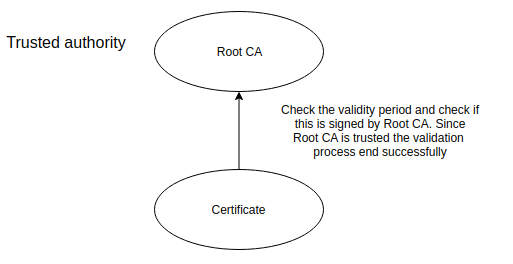
\includegraphics[scale=0.5]{./verification_process.png}
\end{center}
Another task we want to perform is to sign a document and verify the signature with the file author's public key. To reach this goal we should execute this command :
\begin{center}
openssl dgst -sha256 -sign <pvt key> -out <signature>.sha256 <file>,
\end{center}
where pvt key is my private key and file is the file to sign. Naturally will be produced a binary format signature, so for make it human readable we convert it in base64 format via 
\begin{center}
openssl base64 -in <signature>.sha256 -out <signature>.
\end{center}
After signing the document we want to check via issuer's public key if it is the original document or not. Naturally it will be if the hash obtained from the signature is equal to the hash of the original document. Verifying a document via OpenSSL library is very simple :
\begin{center}
openssl dgst -sha256 -verify <owner's pub key> -signature <signature>.sha256 <file>.
\end{center}
This command return "Verified OK" in case of success, otherwise "Verification Failure". Another interesting task is how to convert one certificate from one format to another one. For example, suppose we have the certificate "cert.pem" and we want to convert it to DER format. We just have to execute this command :
\begin{center}
openssl x509 -in cert.pem -inform PEM -out cert.der -outform DER.
\end{center}
\section{HW7 Workflow}
This homework can be seen as a deepening of homework \#6, since we have to take care about request/response for sign/revoke a specific certificate. First of all we need to build a small network formed by two user, one of them will be the Certification Authority. We want to specify that we are using Linux 18.04 as working environment and Vmware software to create two VMs (named client and server) that will talk each other. Once we have set the network, we also need to setup an ssh tunnel between them in order to exchange certificates in a secure way. First of all we need to run ssh server (ssh daemon) and create a user called \textit{user} that will be used to data transfer on each machine. In the previous homework we didn't need to define a configuration file for the Certification Authority, because we have managed simple tasks, but in this case we will define one, since we should revoke some certificates. Lets report this configuration file :
\begin{center}
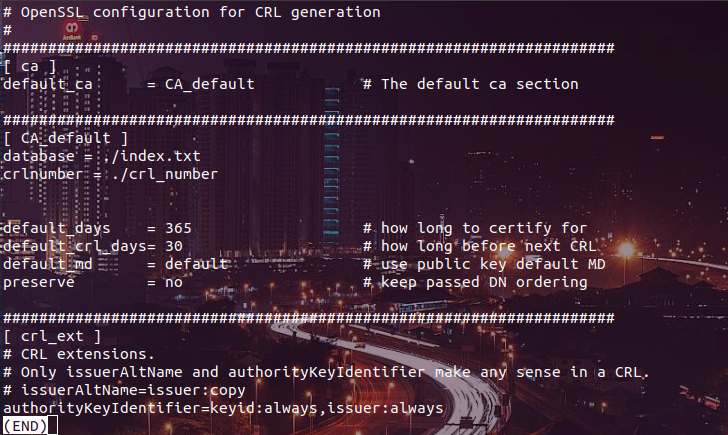
\includegraphics[scale=0.5]{./ca_config_file.png}
\end{center} 
It's a very minimal configuration, since we can see that we have defined one database stored in "index.txt" file, a crl starting number (00 in our case), and other settings like the update frequency of Certification Revocation List. The ca's database will contain all certificates issued in the following format :
\begin{center}
<certification status> <expiration date> <revocation date> <certificate serial number> <certificate filename or "unknown" string> <certificate name>,
\end{center}
where certification status can be valid (V), revoked (R) or expired (E). Lets assume that server is our CA and client a simple user. Lets generate a key pair for the CA (pub\_key.pem,pvt\_key.pem) and a self-signed certificate (ca\_cert.pem). Presently, we want to generate our CRL to keep track about all certificates issued by the server. To do this we just have to execute this command : 
\begin{center}
openssl ca -gencrl -keyfile pvt\_key.pem -cert ca\_cert.pem -out ca\_crl.pem -config ca.conf 
\end{center}
Now lets suppose that client generate a private key using RSA with key's length equals to 2048 bits, extract the public key from this latter and want to sign a certificate via our CA, i.e. 
\begin{center}
private key generation : openssl genpkey -algorithm RSA -out private.pem,\\ public key extraction : openssl rsa -in private.pem -pubout -out public.pem.
\end{center}
Then client need to generate a certificate signing request using his private key :
\begin{center}
openssl req -new -key private.pem -out client\_req.pem.
\end{center}
After that we need to send this request to the server through ssh tunnel, using secure copy utility :
\begin{center}
scp ./req.pem user@server\_address:/requests/,
\end{center}
where server\_address is the server's ip address. We want to underline that the server will run a script that after a specific time interval (we set it to one second) will check if a new request has been received. Once the server discovered that a new request is available then it sign the request with his private key and send back to the subject (client) the signed certificate, i.e.
\begin{center}
Certificate signing : openssl x509 -req -days 360 -in client\_req.pem -CAfile ca\_cert.pem -CAkey pvt\_key.pem -CAcreateserial -out client\_cert.pem,\\Data transfer : scp ./client\_cert.pem user@client\_address:./root/certificates/.
\end{center}
Naturally a certificate can also be revoked from the CA or from the client. Lets take care of the first case. Suppose that the server want to revoke the previously issued certificate; then it will execute the following command :
\begin{center}
openssl ca -revoke client\_cert.pem -keyfile pvt\_key.pem -cert ca\_cert.pem -config ca.conf.
\end{center}
Naturally, we don't need to send data between client and server, because a third party before to trust client should verify if client's certificate was issued by a trusted authority, if it's valid and not revoked. In other words the third party will only have to perform this command :
\begin{center}
openssl verify -crl\_check -CAfile ca\_cert.pem -CRLfile ca\_crl.pem client\_cert.pem,
\end{center}
where ca\_cert.pem, ca\_crl.pem and client\_cert.pem are publicly available. This command in case of failure will return the error code 23 (certificate revoked), otherwise return "OK". An important feature is that once the server revoke a certificate it needs to generate again the CRL, otherwise can arise some security issues due to outdated data (for example using man in the middle attack). The second case is a little bit harder because is the client that want to revoke your own certificate. We can behave like the previous case, but we need to send to the server a useful information to revoke the certificate, for example a file containing the certificate's serial number. From server side with a simple script we can iterate along all certificates and choose only the one to be revoked. Naturally this can be expensive in terms of time complexity, but we can optimize this procedure using an hash map with key-value pairs, where the key represent the certificate's serial number and the value the certificate's filename.
\section{Conclusions}
We have seen that in the first homework we only reasoned about one machine (CA), writing a small script to perform the required tasks. In the second homework we accomplished more difficult activities, like revoke a certificate issued by our CA. We chosen only two VMs for the sake of simplicity, but nothing would change if we had chosen 100 VMs. This feature is really important because with some adroitness we can build a strong protocol for build a CA with all its capabilities, build a client that can require to the server to sign/revoke a particular certificate. These homework are really important to understand how the real world works from the point of view of digital information security.
\end{document}